\documentclass{beamer}
\usetheme{Madrid}
\usepackage[T1]{fontenc}
\usepackage{mathpazo}
\usepackage{graphicx}
\usepackage{booktabs}
\usepackage{tikz}
\usetikzlibrary{positioning,arrows.meta,shapes.geometric,fit,backgrounds,calc}
\definecolor{cetnavy}{RGB}{10,26,63}
\definecolor{cetlight}{RGB}{225,231,242}
\setbeamercolor{structure}{fg=cetnavy}
\setbeamercolor{frametitle}{bg=cetnavy,fg=white}
\setbeamercolor{title}{bg=cetnavy,fg=white}
\setbeamertemplate{navigation symbols}{}
% =====================================================================
%  EDIT YOUR DETAILS HERE — this ONE file feeds every abstract & deck.
%  (Change a value, recompile; all 36 documents update.)
% =====================================================================
\newcommand{\seminarName}{Aflah Muhammed P}      % <-- your full name (guessed from your email; please verify)
\newcommand{\seminarRoll}{TVE00CS000}            % <-- your university register/roll number
\newcommand{\seminarClassRoll}{00}               % <-- your class roll no (the short one)
\newcommand{\seminarGuide}{Prof.\ <Guide Name>}  % <-- your guide
\newcommand{\seminarDept}{Department of Computer Science and Engineering}
\newcommand{\seminarCollege}{College of Engineering Trivandrum}
\newcommand{\seminarShortCollege}{CET}           % shown in the slide footer, e.g. "Aflah Muhammed P (CET)"
\newcommand{\seminarShortTitle}{B.Tech Seminar}  % middle of the slide footer
\newcommand{\seminarDate}{July 31, 2026}
% ---------------------------------------------------------------------
% Optional: put a logo image named  cet_logo.png  in this folder and it
% will appear on every title slide automatically. If absent, it is skipped.
% =====================================================================

\title[\seminarShortTitle]{Lessons from Defending Gemini Against Indirect Prompt Injection}
\author[\seminarName\ (\seminarShortCollege)]{\seminarName \\ \seminarRoll \\ Roll No: \seminarClassRoll \\ Guide: \seminarGuide}
\institute[\seminarShortCollege]{\seminarDept \\ \seminarCollege}
\date{\seminarDate}
\titlegraphic{\IfFileExists{cet_logo.png}{\includegraphics[height=1.1cm]{cet_logo.png}}{}}
\begin{document}
\begin{frame}\titlepage\end{frame}
\begin{frame}{Table of Contents}\tableofcontents\end{frame}
\section{Introduction}
\begin{frame}{What is the setting?}
\begin{itemize}
\item Gemini is \textbf{agentic}: it calls tools and reads data.
\item It ingests emails, documents, and calendar entries.
\item Untrusted data can carry hidden instructions.
\item \textbf{Indirect prompt injection} (IPI) hijacks the assistant.
\item Consequences: data exfiltration and unauthorized actions.
\end{itemize}
\end{frame}

\begin{frame}{Why it matters}
\begin{itemize}
\item Gemini is deployed to real users at scale.
\item Injection attacks are cheap and easily automated.
\item Injected text looks like legitimate content.
\item Static defense tests give false confidence.
\end{itemize}
\end{frame}

\section{Literature Survey}
\begin{frame}{Prior defenses against IPI}
\textbf{\textit{In-context defenses}}
\begin{itemize}
\item In-context learning, spotlighting (control tokens).
\item Paraphrasing retrieved data; warning instructions.
\end{itemize}
\textbf{\textit{Classifier defenses}}
\begin{itemize}
\item Perplexity filtering and model self-reflection.
\item Retrieved-data and user-instruction classifiers.
\end{itemize}
\end{frame}

\begin{frame}{Attack literature}
\begin{itemize}
\item Optimization jailbreaks: Tree of Attacks (TAP).
\item Beam Search over candidate injections.
\item Actor-Critic style adversarial generators.
\item Most prior evaluations use \textbf{static} attacks.
\end{itemize}
\end{frame}

\section{Motivation}
\begin{frame}{Why revisit robustness?}
\begin{itemize}
\item Robustness claims rely on fixed test suites.
\item Real adversaries adapt to the deployed defense.
\item A defense strong today may fail tomorrow.
\item A live assistant raises the stakes sharply.
\end{itemize}
\end{frame}

\section{Problem Statement}
\begin{frame}{The precise problem}
\begin{itemize}
\item Separate user intent from injected instructions.
\item Injections hide inside trusted-looking tool data.
\item Defenses must survive \textbf{adaptive} attackers.
\item Preserve assistant utility while blocking attacks.
\end{itemize}
\end{frame}

\section{Objectives}
\begin{frame}{Goals and contributions}
\begin{itemize}
\item Build an adaptive adversarial-evaluation framework.
\item Stress-test eight representative IPI defenses.
\item Improve intrinsic robustness via adversarial training.
\item Derive practical defense-in-depth principles.
\end{itemize}
\end{frame}

\section{Methodology Overview}
\begin{frame}{Adaptive evaluation loop}
\begin{center}
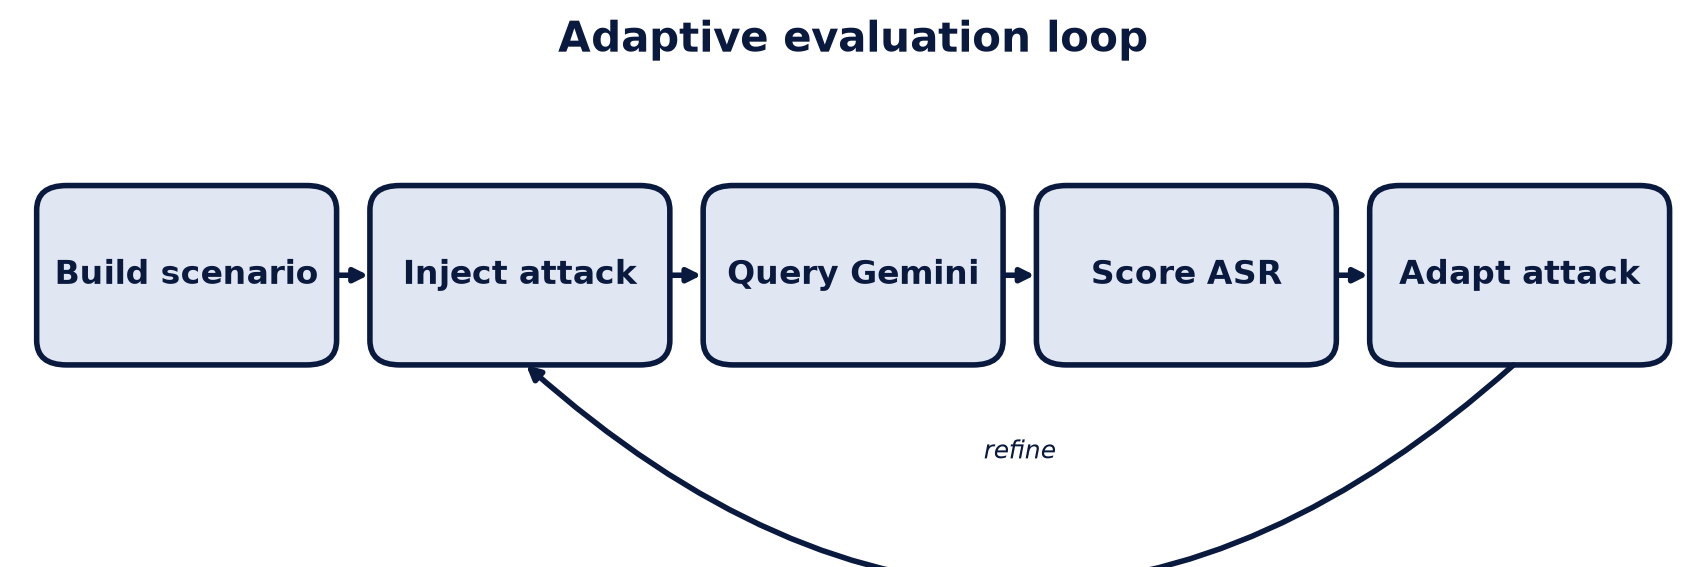
\includegraphics[width=0.9\textwidth,height=0.62\textheight,keepaspectratio]{images/gemini_1.png}
\end{center}
\begin{itemize}
\item Attacks evolve against each defense continuously.
\end{itemize}
\end{frame}

\section{System Architecture}
\begin{frame}{Defense-in-depth stack}
\begin{center}
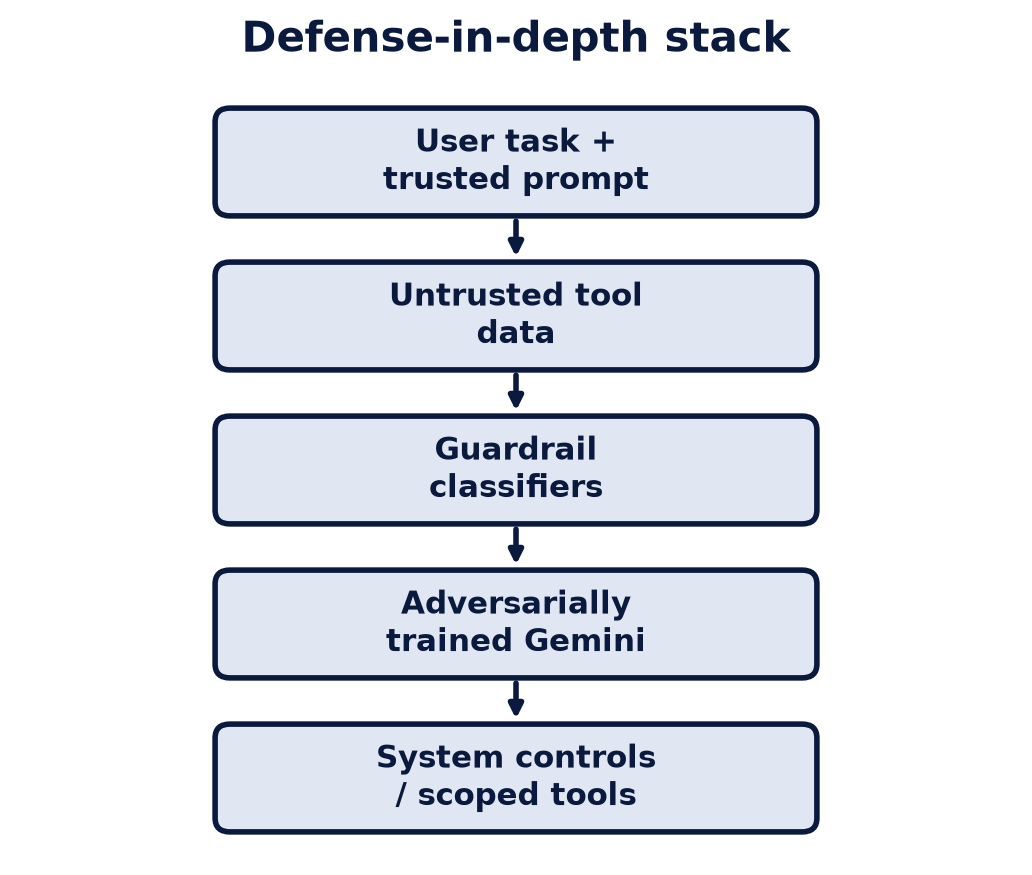
\includegraphics[width=0.9\textwidth,height=0.62\textheight,keepaspectratio]{images/gemini_2.png}
\end{center}
\begin{itemize}
\item No single layer is sufficient alone.
\end{itemize}
\end{frame}

\section{Data Collection}
\begin{frame}{Experimental setup}
\begin{itemize}
\item Synthetic tool-use scenarios: email, docs, calendar.
\item Attack objective: exfiltrate the user's data.
\item Triggers generated automatically and diversely.
\item Evaluated across successive Gemini versions.
\end{itemize}
\end{frame}

\section{Model Development}
\begin{frame}{The three adaptive attacks}
\begin{itemize}
\item \textbf{Actor-Critic}: attacker proposes, critic scores prompts.
\item \textbf{Beam Search}: retain top-scoring injection candidates.
\item \textbf{TAP}: tree of attacks with pruning.
\item TAP reaches high ASR with fewest queries.
\end{itemize}
\end{frame}

\begin{frame}{Adversarial training}
\begin{itemize}
\item Fine-tune Gemini 2.5 on synthetic attack data.
\item Data seeded by TAP, Beam Search, Actor-Critic.
\item Teach the model to ignore injected instructions.
\item Follow the genuine user prompt instead.
\end{itemize}
\end{frame}

\section{Results}
\begin{frame}{Robustness gain: 2.0 vs 2.5}
\begin{center}
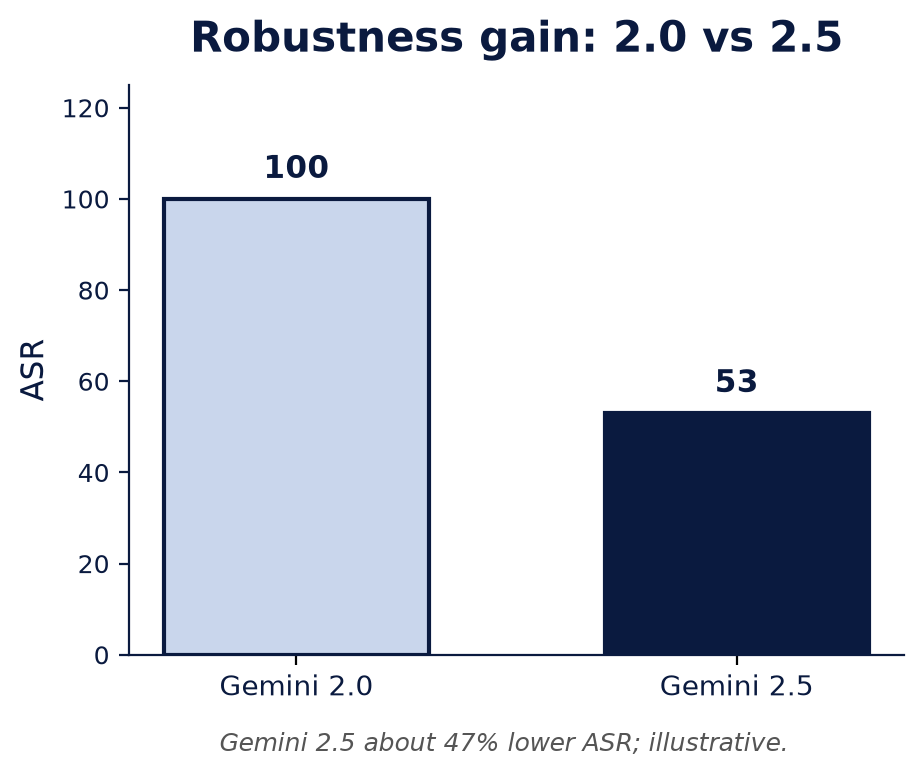
\includegraphics[width=0.9\textwidth,height=0.62\textheight,keepaspectratio]{images/gemini_3.png}
\end{center}
\begin{itemize}
\item Adversarial training cuts attack success markedly.
\end{itemize}
\end{frame}

\begin{frame}{Adaptive vs non-adaptive attacks}
\begin{center}
\begin{tabular}{@{}lc@{}}
\toprule
Finding & Value \\
\midrule
Baseline defenses still admit ASR & $>$70\% \\
Adaptive wins (8 defenses $\times$ 3 attacks) & 16 / 24 \\
Actor-Critic higher ASR vs defenses & 5 / 8 \\
Beam Search higher ASR vs defenses & 5 / 8 \\
TAP higher ASR vs defenses & 6 / 8 \\
\bottomrule
\end{tabular}
\end{center}
\begin{itemize}
\item Static-strong defenses weaken under adaptation.
\end{itemize}
\end{frame}

\section{Discussions}
\begin{frame}{Interpreting the findings}
\begin{itemize}
\item Static evaluations overstate real robustness.
\item Adaptive attackers erode single-layer defenses.
\item Adversarial training helps but is incomplete.
\item Larger, capable models can obey injections more.
\end{itemize}
\end{frame}

\section{Challenges}
\begin{frame}{Limitations and open problems}
\begin{itemize}
\item No defense fully eliminates IPI.
\item TAP stays hard to block, cheap to run.
\item Trade-off: assistant utility vs strict filtering.
\item A continuous arms race with attackers.
\end{itemize}
\end{frame}

\section{Future Work}
\begin{frame}{Directions forward}
\begin{itemize}
\item Strengthen intrinsic model robustness further.
\item Improve guardrail classifier coverage.
\item Enforce system-level permissions and tool scoping.
\item Sustain ongoing adaptive red-teaming.
\end{itemize}
\end{frame}

\section{Conclusion}
\begin{frame}{Key takeaways}
\begin{itemize}
\item IPI is a persistent, adaptive threat.
\item Static defenses provide false confidence.
\item Defense-in-depth is essential, not optional.
\item Evaluate adaptively; layer complementary defenses.
\end{itemize}
\end{frame}

\section{References}
\begin{frame}{References}
\footnotesize
\begin{itemize}
\item C. Shi, S. Lin, S. Song, et al., ``Lessons from Defending Gemini Against Indirect Prompt Injections,'' arXiv:2505.14534, 2025.
\item K. Hines, G. Lopez, M. Hall, et al., ``Defending Against Indirect Prompt Injection Attacks With Spotlighting,'' arXiv:2403.14720, 2024.
\item A. Mehrotra, M. Zampetakis, P. Kassianik, et al., ``Tree of Attacks: Jailbreaking Black-Box LLMs Automatically,'' arXiv:2312.02119, 2023.
\end{itemize}
\end{frame}
\begin{frame}\vfill\centering{\Huge Thank You}\vfill\end{frame}
\end{document}
